\chapter{Visualization Design}

Based on the results of the contextual inquiry, we designed four topic model
visualizations. These visualizations provide different levels of detail so that counselors can
choose the amount of data they see. This design allows the visualizations to be useful
but not unnecessarily overwhelming.

\section{Visual Summary}

The goal of the first two visualizations is to summarize a conversation at a high
level. The topic model data presented are the topics and their proportions that make
up the entire conversation text. For example, one data point might be that the
topic \textit{Rejection} constitutes \textit{50 percent} of the client's side of the conversation. These
visualizations are designed for the user to absorb the data with a quick glance.

\subsection{Topic List}

The first visualization, shown in Figure~\ref{topiclist}, is simply a list of the topic names with
a colored circle next to each name. For each topic's circle, the color corresponds to
the topic and the size corresponds to that topic's proportion of the conversation text.
Topics are ordered by highest proportion first, and only the topics with proportions
over a certain threshold are shown.

\begin{figure}[h]
  \centering
    \fbox{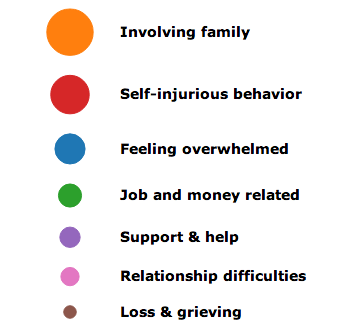
\includegraphics[width=0.6\textwidth]{topiclist.png}}
  \caption{The Topic List visualization provides a visual summary of a conversation
  with a focus on the topics.}
  \label{topiclist}
\end{figure}

A list format was chosen because the focus of this visualization is the topics. We
omit any numbers that emerged from the topic modeling, but the topic names still
need to be ordered to be most useful. Counselors may only care to see the most
dominant topics, and performing a short linear scan of an ordered list allows them to
stop when they please.

The accompanying circles are the visual representations of the topics. They remain
consistent throughout all of the visualizations. Each topic is associated with a color,
and the size of each circle is generally proportional to the percentage of the topic
it represents. These circles allow us to convey the topic model proportions visually
instead of using numbers, which may ease the cognitive load of the visualizations.

We believe the topic list will be useful to counselors when they need a fast reminder
or context. In the case of context switching between parallel conversations with time
gaps, the counselors have already read the conversation text but may need a reference
for recall to jump back into a conversation. For a repeat client, a list of their main
previous issues may be enough context to begin a counseling session.

\subsection{Donut Chart}

The second visualization, shown in Figure~\ref{donutchart}, is a donut chart that displays the
topic proportions as parts of a whole conversation. The included legend is a
mini-version of the topic list, so users are aware that the topics are presented in order. The
slices of the donut are color-coded with our system of topic-color matchings. Mousing
over a slice of the chart or a topic in the legend pops that slice out and replaces the
center text with the topic name and percentage, as shown in Figure~\ref{donutpopout}.

\begin{figure}[h]
  \centering
    \begin{subfigure}[h]{0.75\textwidth}
      \fbox{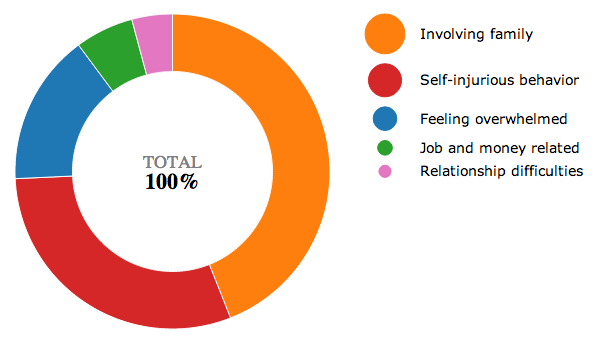
\includegraphics[width=\textwidth]{donutchart.png}}
      \caption{Donut Chart}
      \label{donutchart}
      \vspace{3mm}
    \end{subfigure}
    \begin{subfigure}[h]{0.75\textwidth}
      \fbox{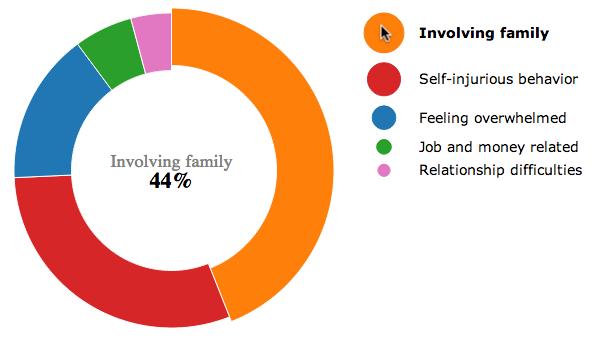
\includegraphics[width=\textwidth]{donutpopout.png}}
      \caption{Donut Chart with mouseover}
      \label{donutpopout}
    \end{subfigure}
  \caption{The Donut Chart visualization provides a visual summary of a conversation
  with more emphasis on the topic proportions.}
\end{figure}

We chose to design a donut chart because pie charts and donuts charts are a
familiar graphic for displaying proportions. This visualization adds to the topic list by
placing some more focus on the proportions in addition to the topic names. Counselors
have access to the specific topic percentage numbers through mouse interaction, but
they are hidden by default to reduce cognitive load.

The donut chart has use cases similar to the topic list, mentioned in the previous
section. We designed both in order to evaluate which one counselors find to be more
helpful for a visual summary.

\section{Visual Indexing}

The topic model data for the next two visualizations dive into more detail. A distinct
set of topics and proportions is given for each client message in the conversation, rather
than one set for the entire conversation. This data allows us to provide information
about where topics are detected within a conversation. We refer to showing this
information visually as \textit{visual indexing} of a conversation. Specifically, selecting a topic
will take the user to the messages visually tagged with that topic in the conversation
transcript. This functionality may be able to greatly reduce the amount of time a
counselor takes to find and read only relevant parts of a transcript. Especially for a
warm transfer or repeat client, the counselor may only want to read the transcript
for information on a specific issue. Automatic visual indexing also represents a form
of note-taking, marking down the important messages so that counselors do not have
to spend time or energy doing it manually.

\subsection{Line Chart}

The line chart visualization in Figure~\ref{linechart} shows topic trends along the timeline of
a conversation. Each topic is displayed as a separate line in this multi-series line
chart, again color-coded by topic. Client message numbers are on the x-axis, and
a topic's proportion in each message is on the y-axis. The user can also click the
\textbf{Show Topic Accumulation} button to show the cumulative topic distribution
on the y-axis instead, shown in Figure~\ref{linechartcumulative}. When the user hovers over a topic in the
legend, the area under that topic line is filled to emphasize the topic.

\begin{figure}[h]
  \centering
    \begin{subfigure}[h]{0.75\textwidth}
      \fbox{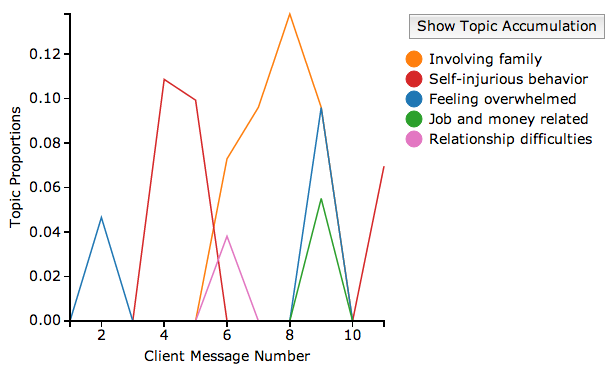
\includegraphics[width=\textwidth]{linechart.png}}
      \caption{Noncumulative Line Chart}
      \label{linechart}
      \vspace{3mm}
    \end{subfigure}
    \begin{subfigure}[h]{0.75\textwidth}
      \fbox{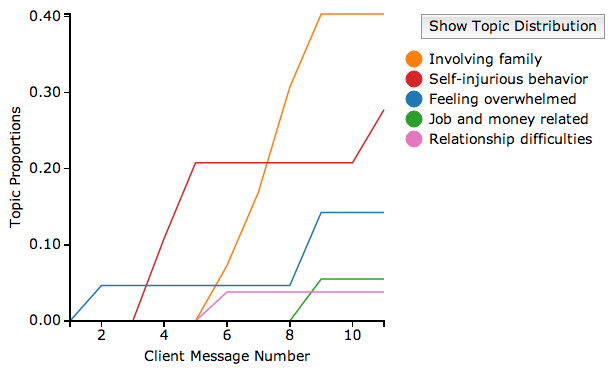
\includegraphics[width=\textwidth]{linechartcumulative.png}}
      \caption{Cumulative Line Chart}
      \label{linechartcumulative}
    \end{subfigure}
  \caption{The Line Chart visualization provides visual indexing of a conversation
  with a focus on topic proportion trends over time.}
\end{figure}

Multi-series line charts are a typical graph for showing multiple trends over time.
Stream graphs are used for similar purposes, but trends can be difficult to comprehend
for individual data series. The focus of this visualization is the change in topic
proportions over time. As outlined in the introduction, we believe topic trends may
help with recall in the situation of context switching with time gaps. Trends may
also alert the counselor to topics on the rise, such as \textit{self-injurious behavior}, that
would compel a certain course of action. Cumulative distributions can be useful for
exhibiting the dominant topics in the conversation encountered so far.

The visual indexing visualizations have an additional interactive aspect. When a
topic is clicked, as in Figure~\ref{linechartpoints}, colored circles appear in the \textbf{Topic Points} column
next to the conversation transcript, and the transcript automatically scrolls to the
first circle. These topic circles act as message tags for visual indexing. Counselors can
use these tags to quickly find the specific messages related to a certain topic. Only
one topic is displayed at a time to reduce cognitive load.

\begin{figure}[h]
  \centering
    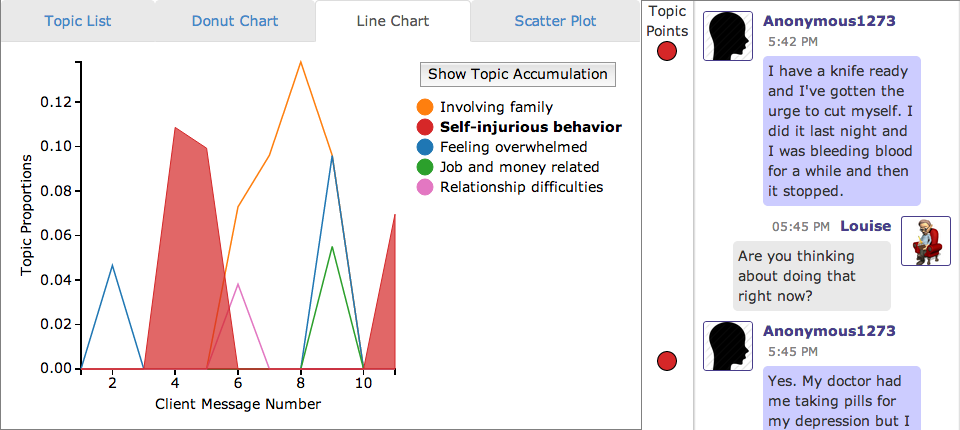
\includegraphics[width=\textwidth]{linechartpoints.png}
  \caption{The Line Chart visualization allows for visual indexing, which shows topic
  points next to messages related to the selected topic in the conversation transcript.}
  \label{linechartpoints}
\end{figure}

\subsection{Scatter Plot}

Figure~\ref{scatterplot} shows the scatter plot visualization. Similar to the line chart, topics are
displayed over time. The x-axis has client message numbers, while the y-axis has
topic names. Each data point in the scatter plot is consistent with our design for a
topic circle: its color corresponds to the topic and its size corresponds to that topic's
proportions. Hovering over a data point or topic name reveals a row border for easy
visual alignment.

\begin{figure}[h]
  \centering
    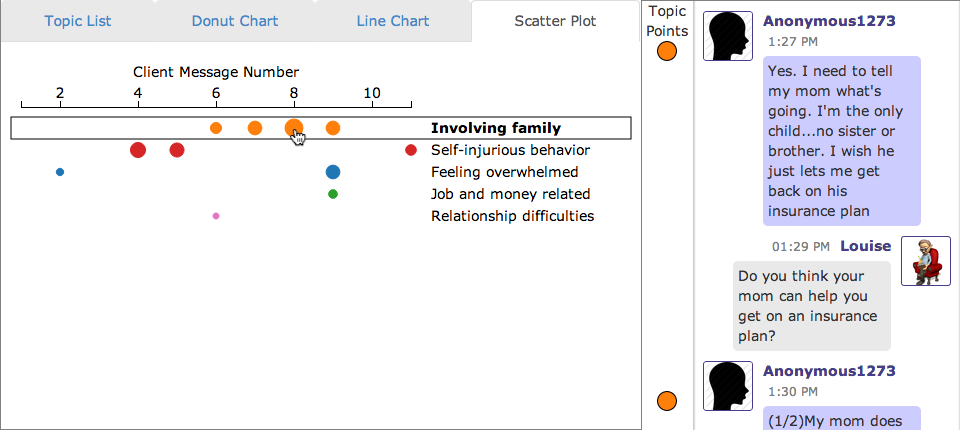
\includegraphics[width=\textwidth]{scatterplot.png}
  \caption{The Scatter Plot visualization is designed for visual indexing, allowing
  users to click on any topic point to automatically scroll to the corresponding message
  in the conversation transcript.}
  \label{scatterplot}
\end{figure}

This design is tailored to visual indexing. We move away from the line chart's
emphasis on topic proportion numbers and concentrate on the existence of a topic in
a message. For counselors searching for any relevant details in the text, proportions
may not matter much. Clicking on any point in the plot will automatically scroll the
conversation transcript to the corresponding tagged message, not just the first one
tagged. This visualization is even more optimized for fast navigation than simply
showing topic points, which the user would still have to scroll through. Counselors
could save a lot of time and energy skimming transcripts without missing relevant
details using this tool.

Like the summary visualizations, the two visual indexing designs have similar
purposes and use the same topic model data. We developed both to evaluate which
one counselors would find more useful, or whether there were aspects of both that are
worthwhile to examine further.
